% Part 2 opening chapter: black-hole horizons. Carries the black-hole thermodynamics paper (25 Feb 2026; 431 PDF lines) in its own order and
% the thermodynamic sections (3, 6, 7) of the information-paradox paper (Feb 2026; 453 lines), both read in full 2026-10-02; the coefficient
% eta and its derivation are Chapter ch:bekenstein (p3_01a_bekenstein.tex); the interpretation of the information paradox is Chapter
% ch:bhinformation (part3/p3_01b_bh_information.tex).
% Corrections applied: PAPER_ERRATA B1 (black-body identity is by construction), B2 (entropy transfer is not the Page curve; 0.646 tau; 1.51e77 bits),
% B3/M1 (M-sigma removed), B6 (no fixed point), B8 (scope), V17 (Smarr 1/2), V20 (S_BH form). Checks: docs/verification/black_holes/BLACK_HOLES_CHECK.md;
% numbers: docs/verification/scripts/verify_bekenstein_bh.py and verify_virial_atoms_to_horizon.py. Figures: figscripts/fig_p2_blackholes.py, fig_p2_bekenstein.py.

\chapter{Black-hole horizons: Bekenstein, Hawking and the price of a bit}\label{ch:blackholes}

\section*{Overview}
IAM's Law (Chapter~\ref{ch:iams_law}) prices every classical record at $k_BT\ln2$ per bit on the nearest encoding surface. For a collapsed
mass the nearest surface is the black hole's own horizon, at the Hawking temperature; that horizon is the place in IAM this chapter reads.
Part~\ref{part:1} ended with the virial half: a system bound by $1/r$ holds half its binding energy as motion, and that half is the irreversible cost of binding. The
next rung of the ladder is the strongest binding there is. A black hole is a surface with a temperature and an entropy, and Landauer's principle can be
applied to it directly. When it is, the same half appears.

The thermodynamic nature of black-hole horizons has been recognized since the foundational work of Bekenstein~\cite{Bekenstein1973} and Hawking~\cite{Hawking1975}. The
Bekenstein--Hawking entropy $S=\kB A/(4\lP^2)$ and the Hawking temperature $T=\hbar c^3/(8\pi GM\kB)$ establish black holes as thermal objects.
Jacobson~\cite{Jacobson1995} derived the Einstein field equations from horizon thermodynamics, showing that gravity is an equation of state. Cai \& Kim~\cite{CaiKim2005}
extended this to FRW spacetimes, demonstrating that the Friedmann equations follow from the first law applied to the apparent horizon. IAM extends this
program by identifying gravitational decoherence as a source of additional informational entropy that, when encoded on the cosmological apparent horizon
via the Cai--Kim procedure, modifies the matter-sector perturbation equations to produce a dual-sector structure ($\mu<1$ for matter, $\Sigma=1$ for photons)
while leaving the background expansion as standard $\Lambda$CDM (Chapters~\ref{ch:virial} and~\ref{ch:theory}).

This chapter applies the same thermodynamic framework to local black-hole horizons. If the cosmic horizon is an encoding surface governed by horizon
thermodynamics, then black-hole horizons must be too --- they are the most efficient encoding surfaces in nature. The chapter sets out the thermodynamics
of black-hole horizons; derives the encoding throughput; shows that the Stefan--Boltzmann luminosity of the horizon and the black-body Hawking luminosity
are one formula; prices the horizon's bits (the Smarr half); follows the entropy that evaporation carries off; constructs the two-horizon framework that
governs the direction of the flow between a black hole and the cold horizon of the universe; and gives the holographic saturation condition for black-hole
formation and its equivalence to the hoop conjecture. Where the famous factor $1/4$ in the Bekenstein--Hawking entropy comes from is
Chapter~\ref{ch:bekenstein}; the same first law applied to the cosmic horizon is Chapter~\ref{ch:virial}. What these results do and do not say about the
information paradox is Chapter~\ref{ch:bhinformation}.

\section{A horizon has a temperature and an entropy}\label{sec:bh_thermo}
Bekenstein (1973)~\cite{Bekenstein1973} argued that a black hole must carry entropy proportional to its area; Hawking (1975)~\cite{Hawking1975} showed that it radiates thermally. For a
Schwarzschild black hole of mass $M$,
\begin{equation}
S_{\rm BH}=\frac{k_Bc^3A}{4G\hbar}=\frac{4\pi Gk_BM^2}{\hbar c},\qquad T_{\rm BH}=\frac{\hbar c^3}{8\pi Gk_BM},\qquad A=\frac{16\pi G^2M^2}{c^4}.
\end{equation}
Every causal horizon has a temperature set by its surface gravity $\kappa$,
\begin{equation}
T=\frac{\hbar\kappa}{2\pi k_Bc},\label{eq:bh_Tuniv}
\end{equation}
with $\kappa=c^4/4GM$ for a black hole, $\kappa=cH$ for the de Sitter horizon of an expanding universe (Gibbons \& Hawking 1977~\cite{GibbonsHawking1977}), and $\kappa=a$ for an
observer with acceleration $a$ (Unruh 1976~\cite{Unruh1976}):
\begin{center}\small\begin{tabular}{lcc}\toprule
horizon & surface gravity $\kappa$ & temperature\\\midrule
black hole & $c^4/(4GM)$ & $T_{\rm BH}=\hbar c^3/(8\pi GM\kB)$\\
cosmic (de Sitter) & $cH$ & $T_{\rm GH}=\hbar H/(2\pi\kB)$\\
Unruh (Rindler) & $a$ & $T_{\rm U}=\hbar a/(2\pi\kB c)$\\\bottomrule
\end{tabular}\end{center}
The $2\pi$ in each case arises from the same source: it is the period of the Euclidean time that makes the horizon smooth (Chapter~\ref{ch:bekenstein},
Section~\ref{sec:bk_twopi}), and it is the same in all three. This is not a coincidence of units --- it is a statement that all horizons are thermal surfaces
obeying the same geometry, and on the reading of this book the same encoding surfaces. \derived\ (formula) \interp\ (encoding reading)

\section{Encoding throughput of a black-hole horizon}\label{sec:bh_throughput}
\subsection{Thermally limited encoding rate}
The maximum rate at which a black-hole horizon can encode information is set by the ratio of the available radiated power to the Landauer cost~\cite{Landauer1961} per
bit:
\begin{equation}
\Gamma_{\rm thermal}=\frac{P}{\kB T_{\rm BH}\ln2}.\label{eq:bh_gamma_def}
\end{equation}
Using the black-body Hawking luminosity~\cite{Hawking1975} $P=\hbar c^6/(15360\pi G^2M^2)$ (Section~\ref{sec:bh_sb}) and the Hawking temperature $T_{\rm BH}=\hbar c^3/(8\pi GM\kB)$:
\begin{equation}
\Gamma_{\rm thermal}=\frac{\hbar c^6/(15360\pi G^2M^2)}{\kB\cdot\hbar c^3/(8\pi GM\kB)\cdot\ln2}=\frac{8\pi}{15360\pi}\,\frac{c^3}{GM\ln2}=\frac{c^3}{1920\,GM\ln2}\ \text{bits\,s}^{-1}.\label{eq:bh_gamma}
\end{equation}
This result is exact for a Schwarzschild black hole in the black-body approximation. The throughput scales inversely with mass: smaller, hotter horizons
encode faster. A $1\,M_\odot$ black hole encodes at $152.5$ bits\,s$^{-1}$. \derived\ (form) \calc\ (value)

\subsection{Numerical values}
Table~\ref{tab:bh_throughput} gives the encoding throughput, the Bekenstein--Hawking entropy in nats ($S_{\rm BH}/\kB=4\pi GM^2/\hbar c$) and in bits, and the
evaporation time $\tau=5120\pi G^2M^3/(\hbar c^4)$ for representative black-hole masses, computed with CODATA 2018 constants~\cite{CODATA2018}. \calc
\begin{table}[htbp]\centering\small
\caption{Hawking temperature, encoding throughput, Bekenstein--Hawking entropy and black-body evaporation time for representative masses (CODATA 2018;
$M_\odot=1.98841\times10^{30}$\,kg; $1\,{\rm yr}=3.15576\times10^7$\,s). \calc}\label{tab:bh_throughput}
\begin{tabular}{lccccc}\toprule
Mass ($M_\odot$) & $T_{\rm BH}$ (K) & $\Gamma$ (bits\,s$^{-1}$) & $S_{\rm BH}$ (nats) & $S_{\rm BH}$ (bits) & $\tau_{\rm evap}$ (yr)\\\midrule
1 & $6.17\times10^{-8}$ & $1.525\times10^{2}$ & $1.049\times10^{77}$ & $1.51\times10^{77}$ & $2.10\times10^{67}$\\
10 & $6.17\times10^{-9}$ & $1.525\times10^{1}$ & $1.049\times10^{79}$ & $1.51\times10^{79}$ & $2.10\times10^{70}$\\
$10^{6}$ & $6.17\times10^{-14}$ & $1.525\times10^{-4}$ & $1.049\times10^{89}$ & $1.51\times10^{89}$ & $2.10\times10^{85}$\\
$10^{9}$ & $6.17\times10^{-17}$ & $1.525\times10^{-7}$ & $1.049\times10^{95}$ & $1.51\times10^{95}$ & $2.10\times10^{94}$\\\bottomrule
\end{tabular}
\end{table}
The evaporation time $\tau_{\rm evap}$ is the time for the black hole to radiate all of its mass; on the reading of this book it is the time to transfer all
locally encoded information to the cosmic horizon via Hawking radiation. \interp

\subsection{Physical interpretation}
$\Gamma_{\rm thermal}$ is the maximum rate at which the horizon processes information --- both encoding new information from incoming gravitational
decoherence and radiating existing information outward via Hawking emission. Section~\ref{sec:bh_bitrate} shows that, in the first law, these two rates are the
same quantity. \interp

\section{The Stefan--Boltzmann luminosity of the horizon}\label{sec:bh_sb}
\subsection{The identity}
The Stefan--Boltzmann law applied to the black-hole horizon is
\begin{equation}
P_{\rm SB}=\sigma_{\rm SB}\,A_{\rm BH}\,T_{\rm BH}^4,
\end{equation}
with $\sigma_{\rm SB}=\pi^2\kB^4/(60\hbar^3c^2)$, $A_{\rm BH}=16\pi G^2M^2/c^4$ and $T_{\rm BH}=\hbar c^3/(8\pi GM\kB)$. Substituting:
\begin{align}
P_{\rm SB}&=\frac{\pi^2\kB^4}{60\hbar^3c^2}\cdot\frac{16\pi G^2M^2}{c^4}\cdot\left(\frac{\hbar c^3}{8\pi GM\kB}\right)^4\notag\\
&=\frac{\pi^2\kB^4}{60\hbar^3c^2}\cdot\frac{16\pi G^2M^2}{c^4}\cdot\frac{\hbar^4c^{12}}{4096\pi^4G^4M^4\kB^4}\notag\\
&=\frac{16}{60\times4096}\,\frac{\hbar c^6}{\pi G^2M^2}=\frac{\hbar c^6}{15360\pi G^2M^2}.\label{eq:bh_PSB}
\end{align}
This is the formula used as the Hawking luminosity in the encoding rate, so
\begin{equation}
\frac{P_{\rm SB}}{P_{\rm Hawking}}=1
\end{equation}
for all masses, verified numerically to 12 significant figures with CODATA 2018 constants (\texttt{verify\_bekenstein\_bh.py}, section J). \derived

\subsection{What the identity says}
The ratio is $1$ by construction: the luminosity $\hbar c^6/(15360\pi G^2M^2)$ is itself the black-body estimate $\sigma_{\rm SB}AT_{\rm BH}^4$, a horizon of area $A$
radiating as a perfect thermal surface at the Hawking temperature. It is therefore a consistency statement, not an independent confirmation. The
emission that quantum field theory in curved spacetime actually predicts differs from it: the spectrum is filtered by greybody factors, the transmission
of each mode through the potential barrier around the hole, and it is summed over the particle species light enough to be emitted (Page 1976~\cite{Page1976}).
These change the numerical coefficient of the luminosity but not its $M^{-2}$ scaling. What the black-body form does show is the physical content the
identity points to: the horizon radiates because it is hot, and its temperature is the price $\kB T\ln2$ of each bit written on it. The black-body formula is
used in this chapter, labelled ``in the black-body approximation'' wherever it sets a number. \derived\ (identity) \interp\ (reading)

\subsection{The Hawking bit rate}\label{sec:bh_bitrate}
The rate at which information departs the black hole via Hawking radiation is
\begin{equation}
\frac{dS_{\rm transfer}}{dt}=\frac{P_{\rm Hawking}}{\kB T_{\rm BH}\ln2}=\frac{c^3}{1920\,GM\ln2}=\Gamma_{\rm thermal}.\label{eq:bh_transfer_rate}
\end{equation}
This is the first law of black-hole thermodynamics read in bits: $c^2|dM/dt|=T_{\rm BH}|dS_{\rm BH}/dt|$, and with $dM/dt=-P/c^2$,
\begin{equation}
-\frac{d}{dt}\Big(\frac{S_{\rm BH}}{\kB\ln2}\Big)=\frac{8\pi GM}{\hbar c\ln2}\cdot\frac{\hbar c^4}{15360\pi G^2M^2}=\frac{c^3}{1920\,GM\ln2},
\end{equation}
so $\Gamma$ is the rate at which the horizon entropy falls. The encoding throughput (Eq.~\eqref{eq:bh_gamma}) and the Hawking emission rate are the same quantity
viewed from two directions. The horizon encodes at precisely the rate it radiates. \derived

\section{The price of the horizon's bits}\label{sec:bh_smarr}

\begin{figure}[htbp]\centering
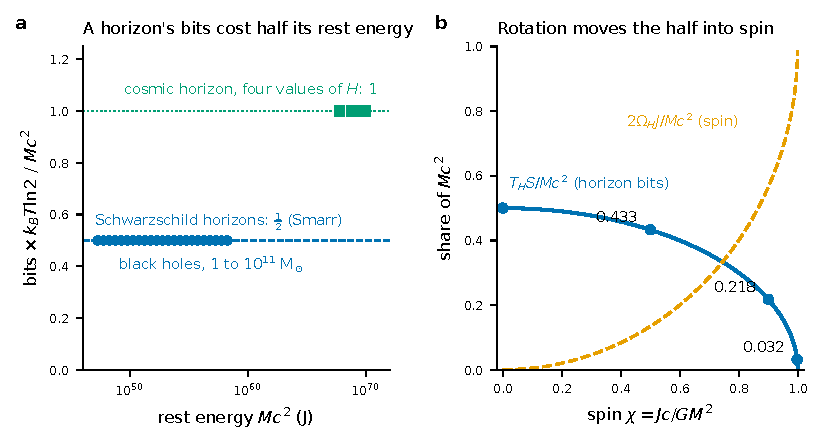
\includegraphics[width=\textwidth]{figures/part3/fig_smarr.pdf}
\caption{(a) The bits of a horizon, $N=S/(k_B\ln2)$, priced at its own temperature, divided by its rest energy. For Schwarzschild black holes from 1 to $10^{11}\,M_\odot$ the ratio is $1/2$ to machine precision ($|\Delta|\lesssim2\times10^{-16}$), the Smarr relation $T_{\rm BH}S_{\rm BH}=\tfrac12Mc^2$; for the cosmic horizon ($H_0=67.4$, Planck 2018, to $10^4$\,km\,s$^{-1}$Mpc$^{-1}$) it is 1, $T_{\rm GH}S=M_Hc^2$. (b) Kerr: $T_{\rm BH}S_{\rm BH}/Mc^2=\sqrt{1-\chi^2}/2$ (0.500, 0.433, 0.218, 0.032 at $\chi=0$, 0.5, 0.9, 0.998) and the spin share $2\Omega_HJ/Mc^2=1-\sqrt{1-\chi^2}$; twice the first plus the second is 1, $Mc^2=2T_{\rm BH}S_{\rm BH}+2\Omega_HJ$. \calc}\label{fig:smarr}
\end{figure}
Count the entropy in bits, $N=S_{\rm BH}/(k_B\ln2)$, and price each one at Landauer's minimum, $k_BT_{\rm BH}\ln2$. The total is
\begin{equation}
N\,k_BT_{\rm BH}\ln2=T_{\rm BH}S_{\rm BH}=\tfrac12Mc^2 ,\label{eq:bh_smarr}
\end{equation}
exactly, for every mass: $0.5000000000$ for one solar mass, for the $4.3\times10^6\,M_\odot$ black hole at the centre of the Galaxy~\cite{Gillessen2009} and for the
$6.5\times10^9\,M_\odot$ black hole in M87~\cite{EHT2019}. In general relativity this is the Smarr relation $Mc^2=2T_{\rm BH}S_{\rm BH}$ (Smarr 1973~\cite{Smarr1973}; Bardeen, Carter \&
Hawking 1973~\cite{BardeenCarterHawking1973}). Read with Landauer's principle it says that half of a black hole's rest energy is the minimum cost of the information on its horizon --- the
same half that the virial theorem gives every $1/r$ system (Chapter~\ref{ch:virial_law}). \derived

Rotation moves energy out of the horizon's bits and into spin. For a Kerr black hole with spin $\chi=Jc/GM^2$, $Mc^2=2T_{\rm BH}S_{\rm BH}+2\Omega_HJ$, and
\begin{equation}
\frac{T_{\rm BH}S_{\rm BH}}{Mc^2}=\frac{\sqrt{1-\chi^2}}{2}:\qquad 0.433\ (\chi=0.5),\quad 0.218\ (\chi=0.9),\quad 0.032\ (\chi=0.998).
\end{equation}
The half belongs to the non-rotating, fully relaxed horizon, as the virial half belongs to the relaxed bound system. \derived

\section{Evaporation and the entropy carried off}\label{sec:bh_evap}
The mass obeys
\begin{equation}
\frac{dM}{dt}=-\frac{P_{\rm Hawking}(M)}{c^2}=-\frac{\hbar c^4}{15360\pi G^2M^2},\label{eq:bh_dMdt}
\end{equation}
which integrates analytically to
\begin{equation}
M(t)^3=M_0^3-\frac{\hbar c^4t}{5120\pi G^2},\qquad \tau_{\rm evap}=\frac{5120\pi G^2M_0^3}{\hbar c^4}.\label{eq:bh_Mt}
\end{equation}
The entropy carried off by the radiation tracks the horizon entropy being transferred to it, at the rate of Eq.~\eqref{eq:bh_transfer_rate} (in this section entropies are counted in bits, $S/\kB\ln2$):
\begin{equation}
\frac{dS_{\rm tr}}{dt}=\Gamma\big(M(t)\big)=\frac{c^3}{1920\,GM(t)\ln2},\qquad
S_{\rm tr}(t)=\int_0^t\frac{c^3}{1920\,GM(t')\ln2}\,dt'.\label{eq:bh_Str}
\end{equation}
Substituting Eq.~\eqref{eq:bh_Mt} and integrating, or directly from the first law of Section~\ref{sec:bh_bitrate},
\begin{equation}
S_{\rm tr}(t)=S_{\rm BH,0}-S_{\rm BH}(t)=S_{\rm BH,0}\Big[1-\Big(1-\frac{t}{\tau_{\rm evap}}\Big)^{2/3}\Big].\label{eq:bh_Str_closed}
\end{equation}
The radiation entropy rises as $M$ decreases (a hotter black hole encodes faster), reaching $S_{\rm BH,0}/2$ at
\begin{equation}
t=\big(1-2^{-3/2}\big)\,\tau_{\rm evap}=0.646\,\tau_{\rm evap},
\end{equation}
and completing the transfer as $M\to0$. The total entropy carried off at $\tau_{\rm evap}$ equals the initial horizon entropy $S_{\rm BH,0}$: in the first law, all bits are
transferred, none created and none destroyed. For a solar-mass black hole, $\tau_{\rm evap}\approx2.1\times10^{58}$\,Gyr, $S_{\rm BH,0}=1.51\times10^{77}$ bits and
$\Gamma=152.5$ bits\,s$^{-1}$. The curve shape is universal; the timescale scales as $M_0^3$ (Fig.~\ref{fig:bh_transfer}). \derived\ (form) \calc\ (values)

\begin{figure}[htbp]\centering
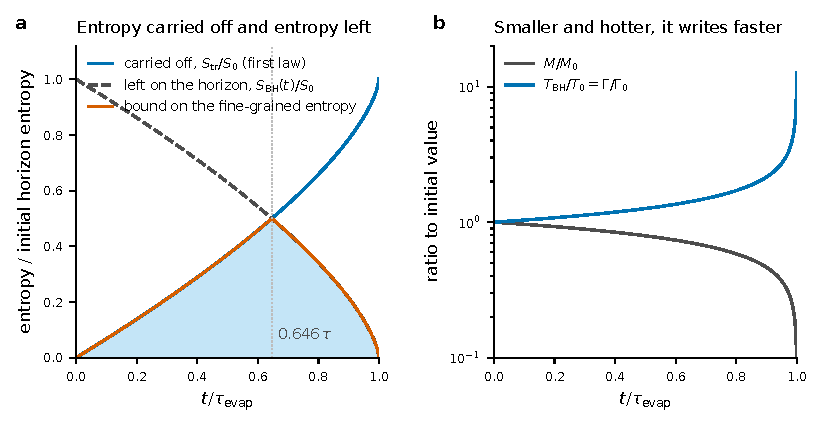
\includegraphics[width=\textwidth]{figures/part3/fig_bh_transfer.pdf}
\caption{Black-body evaporation of a Schwarzschild black hole. (a) Entropy carried off, $S_{\rm tr}/S_0=1-(1-t/\tau)^{2/3}$ (Eq.~\eqref{eq:bh_Str_closed}), and entropy left on the
horizon, $(1-t/\tau)^{2/3}$; they cross at $0.646\,\tau$. The fine-grained entropy of the radiation cannot exceed either, so it lies under the envelope
$\min(S_{\rm tr},S_{\rm BH})$ (shaded); for a unitary evaporation it follows a curve of this shape, rising and then falling to zero (Page~\cite{Page1993}). The first-law transfer itself
(blue) rises monotonically and does not turn over. (b) $M/M_0=(1-t/\tau)^{1/3}$ and $T_{\rm BH}/T_0=\Gamma/\Gamma_0=(1-t/\tau)^{-1/3}$: the hole writes fastest at the end.
\derived\ (form) \calc}\label{fig:bh_transfer}
\end{figure}

\paragraph{This is not the Page curve.} The Page curve~\cite{Page1993} describes how the von Neumann (fine-grained) entropy of Hawking radiation evolves: for a unitary
evaporation it rises, turns over at the Page time and falls back to zero. Equation~\eqref{eq:bh_Str_closed} is a different quantity. It is the coarse-grained, thermal
entropy handed from the horizon to the radiation by the first law, and it rises monotonically to $S_{\rm BH,0}$ with no turnover. What the two curves share is a
bound: the fine-grained entropy of the radiation can be no larger than the coarse-grained entropy it carries, and no larger than the entropy of the
horizon it is entangled with, so it lies under $\min[S_{\rm tr}(t),S_{\rm BH}(t)]$, which in this black-body accounting turns over at the same $0.646\,\tau_{\rm evap}$ (Fig.~\ref{fig:bh_transfer}a).
Whether the true fine-grained entropy follows that envelope, falling to zero, is the information problem itself; the first law cannot decide it.
(Real emission into empty space is irreversible: the radiation's coarse-grained entropy exceeds the horizon entropy it removes, so the crossing, and with it the Page time, comes earlier than in this black-body accounting; for a large hole that emits photons and gravitons, Page finds the maximum of the fine-grained entropy at 53.81\,\% of the evaporation time~\cite{Page2013}, against $64.6\,\%$ here.) The reading of
this result in IAM is Chapter~\ref{ch:bhinformation}. \derived\ (bound) \openprob\ (fine-grained curve)

\section{Two horizons: hot and cold}\label{sec:bh_twohorizons}

\begin{figure}[htbp]\centering
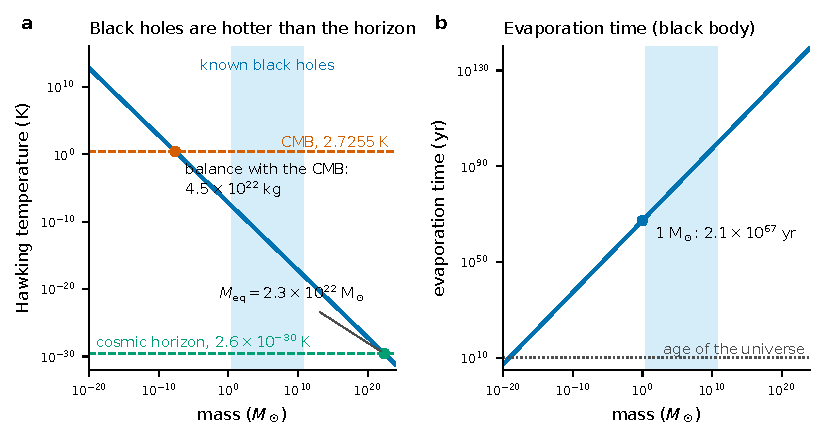
\includegraphics[width=\textwidth]{figures/part3/fig_bh_temperature.pdf}
\caption{(a) Hawking temperature against mass, with the CMB (2.7255\,K) and the cosmic horizon ($T_{\rm GH}=2.6\times10^{-30}$\,K, photon-sector $H_0=67.16$). A black hole balances the CMB at $4.5\times10^{22}$\,kg and the horizon at $M_{\rm eq}=c^3/4GH_0=2.3\times10^{22}\,M_\odot$. Shaded: known black holes, 3 to $6.6\times10^{10}\,M_\odot$. (b) Black-body evaporation time $\tau_{\rm evap}=5120\pi G^2M^3/\hbar c^4$, $2.1\times10^{67}$\,yr for one solar mass; greybody factors change the coefficient, not the scaling. \calc}\label{fig:bh_temperature}
\end{figure}

\subsection{The cosmic horizon temperature}
The universe has its own horizon. The cosmological apparent horizon at $\tilde r_A=c/H$ has the Gibbons--Hawking temperature~\cite{GibbonsHawking1977}
\begin{equation}
T_{\rm GH}=\frac{\hbar H}{2\pi\kB}.\label{eq:bh_TGH}
\end{equation}
At the present epoch ($H_0=67.4$\,km\,s$^{-1}$\,Mpc$^{-1}$, Planck 2018~\cite{Planck2018VI}), $T_{\rm GH}=2.66\times10^{-30}$\,K ($2.65\times10^{-30}$\,K at the photon-sector $H_0=67.16$), many orders of magnitude below any black-hole Hawking temperature. \calc

\subsection{Net radiation between two thermal horizons}
Both the black-hole horizon and the cosmic horizon are thermal surfaces. In the black-body approximation the net radiative power between them is
\begin{equation}
P_{\rm net}=\sigma_{\rm SB}\,A_{\rm BH}\big(T_{\rm BH}^4-T_{\rm GH}^4\big).\label{eq:bh_Pnet}
\end{equation}
Three regimes exist: (1) $T_{\rm BH}>T_{\rm GH}$ ($M<M_{\rm eq}$): standard Hawking radiation, and information flows from the black hole to the cosmic horizon;
(2) $T_{\rm BH}=T_{\rm GH}$ ($M=M_{\rm eq}$): thermal equilibrium, no net flow; (3) $T_{\rm BH}<T_{\rm GH}$ ($M>M_{\rm eq}$): net absorption from the cosmic horizon. \derived

\subsection{Equilibrium mass}
Setting $T_{\rm BH}=T_{\rm GH}$,
\begin{equation}
\begin{gathered}\frac{\hbar c^3}{8\pi GM_{\rm eq}\kB}=\frac{\hbar H}{2\pi\kB}\quad\Longrightarrow\quad M_{\rm eq}=\frac{c^3}{4GH}=2.32\times10^{22}\,M_\odot\\(H_0=67.4\ \text{km\,s}^{-1}\text{Mpc}^{-1},\ \text{Planck 2018}).\end{gathered}\label{eq:bh_Meq}
\end{equation}
\derived\ At the photon-sector $H_0=67.16$ it is $2.33\times10^{22}\,M_\odot$ \calc. Table~\ref{tab:bh_meq} gives $M_{\rm eq}$ and $T_{\rm GH}$ at representative cosmological epochs.
\begin{table}[htbp]\centering\small
\caption{Thermal equilibrium mass $M_{\rm eq}=c^3/(4GH)$ and Gibbons--Hawking temperature $T_{\rm GH}$ at representative epochs. Hubble parameter
$H(z)=H_0\sqrt{\Omega_m(1+z)^3+\Omega_\Lambda+\Omega_r(1+z)^4}$ with $H_0=67.4$\,km\,s$^{-1}$\,Mpc$^{-1}$, $\Omega_m=0.315$, $\Omega_r=9.2\times10^{-5}$ (photons at 2.7255\,K and three neutrino species, $N_{\rm eff}=3.046$), flat~\cite{Planck2018VI}.
The largest known black hole (TON~618, $6.6\times10^{10}\,M_\odot$~\cite{Shemmer2004}) is far below $M_{\rm eq}$ at all epochs shown. At $z=10^{10}$ the plasma, at about 1.7\,MeV, still holds electron--positron pairs, which the $(1+z)^4$ scaling of $\Omega_r$ leaves out; with them $H$ is about 9\,\% lower and $M_{\rm eq}\approx2.65\times10^{4}\,M_\odot$. The conclusion is unchanged. \calc}\label{tab:bh_meq}
\begin{tabular}{lccc}\toprule
epoch & $H$ (s$^{-1}$) & $T_{\rm GH}$ (K) & $M_{\rm eq}$ ($M_\odot$)\\\midrule
$z=0$ & $2.18\times10^{-18}$ & $2.66\times10^{-30}$ & $2.32\times10^{22}$\\
$z=1$ & $3.91\times10^{-18}$ & $4.75\times10^{-30}$ & $1.30\times10^{22}$\\
$z=10^3$ & $4.41\times10^{-14}$ & $5.37\times10^{-26}$ & $1.15\times10^{18}$\\
$z=10^6$ & $2.10\times10^{-8}$ & $2.55\times10^{-20}$ & $2.42\times10^{12}$\\
$z=10^{10}$ & $2.10\times10^{0}$ & $2.55\times10^{-12}$ & $2.42\times10^{4}$\\\bottomrule
\end{tabular}
\end{table}
All astrophysical black holes at all cosmological epochs shown satisfy $M\ll M_{\rm eq}$: every black hole is hotter than the cosmic horizon. The cosmic-horizon
bath correction to the emission, $(T_{\rm GH}/T_{\rm BH})^4$, is $3.4\times10^{-90}$ for a solar-mass black hole today, so against the cosmic horizon alone Hawking radiation
proceeds at the full uncorrected rate to extraordinary precision. \calc

\subsection{The sky a black hole sits in}
The sky a black hole actually sits in is not at $T_{\rm GH}$, though: it is filled with the cosmic microwave background at $T_{\rm CMB}=2.7255$\,K~\cite{Fixsen2009}. A
solar-mass black hole has $T_{\rm BH}=61.7$\,nK, $4.4\times10^{7}$ times colder, so today it absorbs about $(T_{\rm CMB}/T_{\rm BH})^4\approx4\times10^{30}$
times more radiation than it emits (equal-area black-body estimate) and grows. A black hole is in balance with the CMB at
\begin{equation}M_{\rm CMB}=\frac{\hbar c^3}{8\pi Gk_BT_{\rm CMB}}=4.5\times10^{22}\ \text{kg}\approx0.6\,\text{lunar masses};\end{equation}
only lighter holes, which no known process forms today, are net emitters now. Every stellar and supermassive black hole begins to lose mass only after
the expansion has cooled the CMB below its own temperature: for one solar mass the scale factor must grow another $4.4\times10^{7}$-fold (17.6 e-folds). From then on,
energy and entropy flow from the hot local horizon to the cold cosmic one at the rate $\Gamma$, over times of $10^{67}$ years and longer. \calc

\subsection{Information flow direction}
The thermodynamic flow is unambiguous: information encoded on local (hot) black-hole horizons radiates outward toward the global (cold) cosmic horizon. The
sequence is: (1) gravitational decoherence produces information locally; (2) the information is encoded on the nearest available horizon --- the black hole;
(3) the black hole radiates at $T_{\rm BH}$, transferring information to the bulk; (4) the information is ultimately re-encoded on the cosmic horizon at $T_{\rm GH}$.
The timescales for step (3) are $\sim10^{67}$\,yr and above (Table~\ref{tab:bh_throughput}), and step (3) begins in earnest only once the CMB has cooled below $T_{\rm BH}$, so
astrophysical black holes are effectively permanent local storage on cosmological timescales. \interp\ (steps 1, 2, 4) \derived\ (direction of the flow)

\section{When a horizon forms}\label{sec:bh_formation}
\subsection{Saturation as the formation criterion}
In IAM, a black hole forms when the local information production from gravitational decoherence saturates the holographic bound on the bounding
surface:
\begin{equation}
\frac{S_{\rm info}(R)}{\kB A(R)}\ge\frac{1}{4\lP^2},\label{eq:bh_saturation}
\end{equation}
where $S_{\rm info}$ is the information produced by decoherence within radius $R$ and $A=4\pi R^2$ is the bounding surface area. \conjecture

\subsection{Equivalence to the hoop conjecture}
Thorne's hoop conjecture~\cite{Thorne1972} says a black hole forms when mass $M$ is compressed into a region with circumference $C\le4\pi GM/c^2$. The saturation
condition with $S_{\rm info}=S_{\rm BH}=4\pi G\kB M^2/(\hbar c)$ at the Schwarzschild radius $R_s=2GM/c^2$, where the holographic bound
$S/A\le k_B/(4\ell_P^2)$~\cite{Bousso2002} is met exactly, gives
\begin{equation}
\frac{4\pi Gk_BM^2/(\hbar c)}{4\pi(2GM/c^2)^2}=\frac{k_Bc^3}{4\hbar G}=\frac{k_B}{4\ell_P^2}.\label{eq:bh_hoop}
\end{equation}
The conditions are identically satisfied. The hoop conjecture is the holographic bound expressed in geometric language; IAM's saturation condition is the
hoop conjecture expressed in informational language. The same mathematics, with the thermodynamic reason made explicit: a black hole forms when the
local information production saturates the surface's encoding capacity. \derived\ (Eq.~\eqref{eq:bh_hoop}) \interp\ (reading)

\subsection{Early universe: encoding on black-hole horizons}
IAM's activation function $E(a)=\exp(1-1/a)$ (Chapter~\ref{ch:iams_law}) tracks the cosmic horizon's informational entropy. At early times ($E(a)\approx0$),
information is encoded primarily on local black-hole horizons, not on the small cosmic horizon. As the universe expands and large-scale structure formation
produces distributed decoherence, the cosmic horizon grows and takes over as the dominant encoder. On this reading rapid early black-hole formation is
thermodynamically favoured --- the early universe needs encoding surfaces, and black holes are the most efficient ones available before the cosmic horizon
grows --- and the massive early black holes found by JWST are expected rather than anomalous. The same reading is given from the cosmological
side in Chapter~\ref{ch:theoryinterp}. \conjecture

\subsection{Primordial black holes}
During radiation domination, electromagnetic interactions decohere particles far faster than gravity acts. Gravitational decoherence is subdominant. IAM
therefore does not modify the primordial black-hole formation threshold $\delta_c\approx1/3$: primordial black holes form by the standard mechanism (Carr
1975~\cite{Carr1975}; Carr et al.\ 2010~\cite{Carr2010}). IAM's contribution to structure formation begins after recombination ($z\sim1100$), when photon decoupling makes
gravitational decoherence the dominant irreversible information source. \interp

\subsection{Seed masses from an information budget}
After recombination, for collapsing halos at $z\sim20$--30, the black-hole mass whose horizon holds a given information budget follows from inverting
$S_{\rm BH}/\kB=4\pi GM^2/(\hbar c)$:
\begin{equation}
M_{\rm BH}=\frac{m_{\rm Pl}}{2\sqrt\pi}\sqrt{S_{\rm collapse}},\label{eq:bh_seed}
\end{equation}
where $S_{\rm collapse}$ (in nats) is the total irreversible gravitational information produced during collapse and $m_{\rm Pl}=\sqrt{\hbar c/G}$ is the Planck mass.
\derived\ (inversion)
\begin{table}[htbp]\centering\small
\caption{Black-hole mass whose horizon holds a given collapse entropy, Eq.~\eqref{eq:bh_seed}. The mass is set by the information content of the collapse, not by
accretion history. Computing the collapse entropies themselves is the next step. \calc\ (inversion) \openprob\ ($S_{\rm collapse}$)}\label{tab:bh_seed}
\begin{tabular}{lcl}\toprule
$S_{\rm collapse}$ (nats) & $M_{\rm BH}$ ($M_\odot$) & class\\\midrule
$10^{77}$ & $0.98$ & stellar mass\\
$10^{83}$ & $9.8\times10^{2}$ & intermediate mass\\
$10^{89}$ & $9.8\times10^{5}$ & supermassive\\
$10^{95}$ & $9.8\times10^{8}$ & ultra-massive\\\bottomrule
\end{tabular}
\end{table}
The mass scales with $\sqrt{S_{\rm collapse}}$, so each six-order-of-magnitude increase in information content produces a three-order-of-magnitude increase in seed
mass. If the collapse entropy can be computed, this provides a formation channel for massive early black holes that requires neither super-Eddington
accretion nor exotic seed mechanisms --- only the information budget of the collapse. \conjecture\ The collapse entropy that such seed masses require is taken as given here; its derivation is open, and until it is done Table~\ref{tab:bh_seed} is an inversion of the area law rather than a prediction. \openprob

\paragraph{How close a remnant is to its limit.} Every compact remnant is held up against gravity by a pressure that can only support so much
mass: electron degeneracy up to the Chandrasekhar mass~\cite{Chandrasekhar1931} ($1.44\,M_\odot$; $1.456\,M_\odot$ for $\mu_e=2$ from the constants alone), neutron
degeneracy and nuclear forces up to the Tolman--Oppenheimer--Volkoff limit~\cite{Tolman1939,OppenheimerVolkoff1939} (taken here as $\approx2.3\,M_\odot$; a recent multimessenger
inference gives $2.25^{+0.08}_{-0.07}\,M_\odot$~\cite{Fan2024}). On the same gauge as every other system in this book, $A$ is the remnant's mass over the typical remnant of its kind as built
(white dwarfs $0.6\,M_\odot$, the measured mean of $0.593\,M_\odot$ for DA white dwarfs~\cite{Kepler2007}; neutron stars $1.4\,M_\odot$), so $A=1$ sits in the middle. The far right is where the surface is
full: no pressure can hold, a horizon forms and the black hole begins (Fig.~\ref{fig:stargauge}). \observed\ (masses) \calc\ ($A$)
\begin{center}\small\begin{tabular}{lccc}\toprule
remnant & mass ($M_\odot$) & $A$ & surface full at\\\midrule
the Sun's future white dwarf~\cite{Sackmann1993} & 0.54 & 0.90 & 2.40\\
Procyon B (wide binary)~\cite{Bond2015} & 0.592 & 0.99 & 2.40\\
Sirius B (wide binary)~\cite{Bond2017} & 1.02 & 1.70 & 2.40\\
IK Pegasi B (21.7-day binary)~\cite{Landsman1993} & 1.15 & 1.92 & 2.40\\
typical neutron star & 1.4 & 1.00 & 1.64\\
PSR J0740+6620~\cite{Fonseca2021} & 2.08 & 1.49 & 1.64\\\bottomrule
\end{tabular}\end{center}
A white dwarf that is isolated or in a wide binary has nothing to accrete, so it stays where it is; only a remnant that gains mass, from a close companion
as it evolves or from a collapsing core, moves right. What stops the star at the far right is ordinary physics, the pressure failing. What forms there is the object that holds the most entropy any
region of that size and energy can hold: a black hole saturates the Bekenstein bound~\cite{Bekenstein1981}. This is the one gauge in the book where the far-right line is
already known from physics: derived from the constants for white dwarfs (the Chandrasekhar mass) \derived\ and inferred to a few per cent for neutron stars ($2.25^{+0.08}_{-0.07}\,M_\odot$~\cite{Fan2024}) \observed; for cells the corresponding line is still to be measured (Chapter~\ref{ch:onegauge}, Part~\ref{part:5}) \openprob.
\begin{figure}[htbp]\centering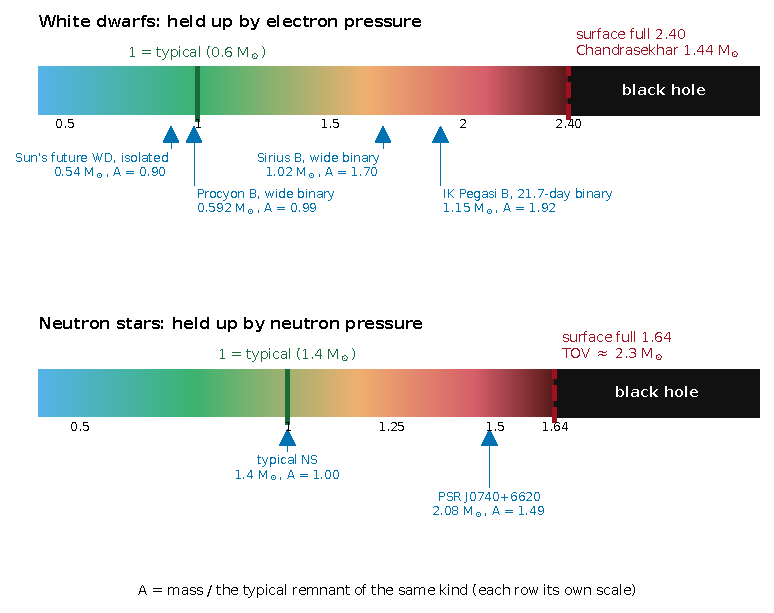
\includegraphics[width=\textwidth]{figures/part3/star_gauge.pdf}
\caption{Compact stars on the same gauge: mass over the typical remnant of the same kind ($0.6\,M_\odot$ white dwarfs, $1.4\,M_\odot$ neutron stars).
Dashed: the surface is full at the Chandrasekhar mass ($1.44\,M_\odot$, $A=2.40$) or the TOV limit ($\approx2.3\,M_\odot$, $A\approx1.64$); beyond,
a black hole. Each row has its own scale. \calc}\label{fig:stargauge}\end{figure}

\section{Two regimes of one mechanism}\label{sec:bh_regimes}
IAM's feedback loop --- decoherence $\to$ information production $\to$ Landauer cost $\to$ horizon encoding $\to$ modified expansion --- operates in two regimes. In
the cosmological (self-regulating) regime, distributed decoherence produces information gradually, encoded on the growing cosmic horizon. Expansion dilutes
matter, slowing further collapse. The feedback reaches equilibrium, producing $\mu<1$, $\Sigma=1$. In the collapse (runaway) regime, concentrated decoherence
produces information explosively in a contracting region. Local encoding capacity saturates. The feedback runs away, producing a new horizon.
\begin{center}\small\begin{tabular}{lll}\toprule
 & cosmological (self-regulating) & collapse (runaway)\\\midrule
decoherence rate & gradual, from structure formation & explosive, from gravitational collapse\\
information encoding & distributed on the cosmic horizon & concentrated on a local horizon\\
pressure release & cosmic expansion dilutes matter & no valve --- gravity wins locally\\
result & $\mu<1$, $\Sigma=1$, $E(a)\to e$ & a new encoding surface: a black hole\\\bottomrule
\end{tabular}\end{center}
Same physics. Same mechanism. Different boundary conditions. \interp\ The cosmological regime is worked out in Chapters~\ref{ch:virial} and~\ref{ch:theory}; both regimes
are read together in Chapter~\ref{ch:theoryinterp}.

\paragraph{Gravity in, gravity out.} In both columns of the table gravity is the drive and the output. At the cosmic scale, matter collapsing under
gravity writes the records, and their accumulated cost modifies the matter-sector expansion. At the black-hole scale, gravitational binding drives
the record to the saturation point, and at saturation a new encoding surface forms: the horizon. With $E_{\rm drive}=Mc^2$ at $T_{\rm BH}$ the
drive ratio is $\mathcal M=Mc^2/k_BT_{\rm BH}=8\pi(M/m_P)^2=2S_{\rm BH}/k_B$, with $m_P=\sqrt{\hbar c/G}$: the Smarr relation again, and
$2.1\times10^{77}$ for one solar mass ($3.0\times10^{77}$ in Landauer units, $\mathcal M/\ln2$; Chapter~\ref{ch:iams_law}). \derived{} Read this way, IAM is not a model of gravity plus
information; it is one process, gravity writing records, seen at different scales of $\mathcal M$. \interp


\section{What can be tested}\label{sec:bh_tests}
\begin{table}[htbp]\centering\small
\caption{Results and tests of the two-horizon framework.}\label{tab:bh_tests}
\begin{tabular}{p{0.264\textwidth}p{0.322\textwidth}p{0.313\textwidth}}\toprule
result & value & status and test\\\midrule
encoding throughput & $\Gamma=c^3/(1920\,GM\ln2)$ (black body) & \derived; constrains the black-hole information-processing rate; greybody factors change the coefficient\\
$P_{\rm SB}=P_{\rm Hawking}$ & identity in the black-body approximation, Eq.~\eqref{eq:bh_PSB} & \derived\ by construction; not a test\\
every black hole hotter than the cosmic horizon & $M_{\rm eq}>10^{22}\,M_\odot$ at $z=0$ (Table~\ref{tab:bh_meq}) & \calc; net emission begins only when $T_{\rm CMB}<T_{\rm BH}$\\
no change to primordial black-hole formation & $\delta_c$ unchanged & \interp; consistent with primordial black-hole constraints\\
early massive black holes from an information budget & Table~\ref{tab:bh_seed} & \conjecture; needs $S_{\rm collapse}$; JWST\\
lensing-to-hydrostatic cluster mass & $1/\mu(z)$: $1.158$ at $z=0$, falling with $z$ & \prediction; eROSITA and Euclid clusters (Chapter~\ref{ch:threeway})\\\bottomrule
\end{tabular}
\end{table}

\section{Scope, and what the informational entropy is}\label{sec:bh_scope}
The present treatment is interpretive and restricted to semiclassical horizon thermodynamics. A complete microscopic derivation of the informational
entropy functional from quantum gravity remains an open problem. \openprob\ The framework does not claim to replace the Bekenstein--Hawking entropy nor to
resolve the black-hole information paradox. Instead, it provides a phenomenological extension aimed at understanding the thermodynamic role of bulk
decoherence within classical gravity.

The informational entropy introduced in IAM is not proposed as a correction to the Bekenstein--Hawking area law. The geometric entropy $S_{\rm BH}=\kB A/4\lP^2$
continues to encode the microscopic horizon degrees of freedom as in standard semiclassical gravity. The additional term represents a coarse-grained entropy
associated with irreversible bulk processes (gravitational decoherence and classicalization). It therefore reflects a macroscopic accounting of
information production, not an independent set of fundamental horizon microstates. This distinction avoids double counting and preserves the validity of
the standard black-hole entropy formula. The term can be written as a covariant scalar functional that vanishes in exact stationary spacetimes, enters
dynamical settings as a boundary contribution proportional to the horizon temperature, preserves the Bianchi identity and introduces no additional
propagating degrees of freedom; its action is given in Chapter~\ref{ch:theory}. \interp

\section{Where the 1/4 comes from}\label{sec:bh_quarter}
Jacobson (1995)~\cite{Jacobson1995} obtained the Einstein equations from $\delta Q=T\,\delta S$ on local Rindler horizons, with $T=\hbar\kappa/(2\pi k_Bc)$ and $S=\kB\eta A$. The
Clausius relation holds for every null direction only if
\begin{equation}
\frac{\hbar\eta}{2\pi}=\frac{c^3}{8\pi G}\qquad\Longrightarrow\qquad\eta=\frac{c^3}{4\hbar G}=\frac{1}{4\ell_P^2}.
\end{equation}
The $1/4$ is the ratio of two geometric numbers: the $2\pi$ period of the Euclidean horizon (Bisognano \& Wichmann 1976~\cite{BisognanoWichmann1976}; Unruh 1976~\cite{Unruh1976}) and the $8\pi$ of the
field equations ($4\pi$ from Gauss's law in three dimensions, doubled by the trace structure of $G_{ab}$). Given Newton's constant, nothing else enters.
The same ratio gives one unit of entropy, $k_B$, per $4\ell_P^2$ of horizon at every surface gravity; one bit takes $4\ln2\,\ell_P^2$. What thermodynamics cannot supply is why a smallest area $\ell_P^2=\hbar G/c^3$
exists at all; that is a question about the microstructure of spacetime. The derivation, step by step, is Chapter~\ref{ch:bekenstein}. \derived

\section{From the black hole to the universe}\label{sec:bh_universe}
Black-hole horizons treated as thermal encoding surfaces within horizon thermodynamics yield three exact results in the black-body approximation: the
encoding throughput $\Gamma_{\rm thermal}=c^3/(1920\,GM\ln2)$, the identity of the Stefan--Boltzmann and Hawking luminosities, and the monotonic flow of
energy and entropy from local hot horizons to the global cold cosmic horizon. To these the Smarr relation adds the price of the horizon's bits, half the
rest energy. The thermal equilibrium mass $M_{\rm eq}=c^3/(4GH)$ exceeds all astrophysical black holes at every cosmological epoch, so every real black hole
is hotter than the cosmic horizon throughout cosmic history; against the warmer CMB they grow today and begin to radiate only in the far future. The hoop
conjecture is the holographic bound in geometric language; the saturation condition is the hoop conjecture in informational language.

A black hole's horizon carries entropy $A/4\ell_P^2$, sits at temperature $\hbar\kappa/2\pi k_Bc$, and holds half its mass-energy as the Landauer cost of its
bits. The horizon of the universe obeys the same first law. Jacobson and Cai \& Kim~\cite{Jacobson1995,CaiKim2005} showed that applying $-dE=T\,dS$ at the cosmic apparent horizon returns the
Friedmann equations. Chapter~\ref{ch:virial} adds to that first law the entropy written as matter decoheres, and the virial half fixes how much of the matter
density enters it: $\beta_m=\Omega_m/2$. The same mechanism that modifies cosmic growth ($\mu<1$, $\Sigma=1$) creates the strongest gravitational objects in the
universe, differing only in boundary conditions. One mechanism, two regimes, every scale. \interp

The formation of a horizon as the point where no outer surface can hold the records, and what this picture says about the information paradox, are taken
up in Chapter~\ref{ch:bhinformation} and in Part~\ref{part:5} (Chapter~\ref{ch:theoryinterp}).

A black hole is the cleanest place to watch the price at work: the Smarr relation is the cost of the horizon's bits. A relativist can take that reading to any horizon, and a reader who wants the numbers can recompute every one of them from the repository.
